\section{随机反相器、乘法器和隔离器}

要将表示形式 (ii) 中的量乘以 $-1$，只需交换 UP 和 DOWN 线路. 在表示形式 (i) 中，逻辑反相器（其输出为其输入的补）执行相同的功能. 考虑其输出为 ON 的概率 $\mathbf{p}^{\prime}$ 与其输入为 ON 的概率 p 之间的关系. 即

\[
p^{\prime} = 1 - p \tag{5}
\]

由公式 (1)，这些概率与它们所表示的量之间的关系为：

\[
\begin{array}{l}
p = \frac{1}{2} E / V + \frac{1}{2} \\
p^{\prime} = \frac{1}{2} E^{\prime} / V + \frac{1}{2}
\end{array}
\]

因此

\[
\mathbf{E}^{\prime} = -\mathbf{E} \tag{8}
\]

将一个量与另一个量相乘可以通过表示形式 (i) 中的反相异或门以及表示形式 (ii) 中的一对类似门来实现. 图 3(i) 和 3(ii) 分别展示了这些随机乘法器在 NAND 逻辑中的实现.

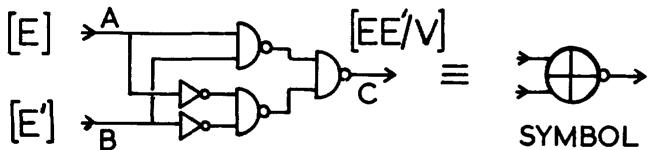
\includegraphics[width=0.6\textwidth, height=7cm, keepaspectratio]{images/006cd21d90ed91a778330bc2c7410063641a619aaeebcfebb6a1829dec084b21.jpg}\\
(i) $C = A.B \vee \overline{A}.\overline{B}$

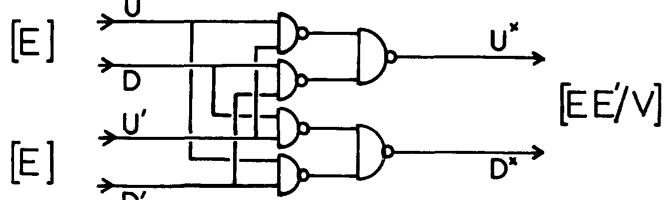
\includegraphics[width=0.6\textwidth, height=7cm, keepaspectratio]{images/87b5233b7b2642581fc555b9961d8e8aaeb4f0652acf86b532de3129ae1a8def.jpg}\\
$U^* = U.U^{\prime} \vee D.D^{\prime}$ (ii)\\
$D^* = U.D^{\prime} \vee D.U^{\prime}$

图 3---随机乘法器

检验图 3 中门的输入和输出概率之间的关系，可确认确实执行了乘法运算. 对于 3(i)：

\[
\begin{array}{l}
\mathrm{p}(\mathrm{C}) = \mathrm{p}(\mathrm{A}) \mathrm{p}(\mathrm{B}) + (1 - \mathrm{p}(\mathrm{A})) (1 - \mathrm{p}(\mathrm{B})) \\
\text{由公式 (1)：}
\end{array} \tag{9}
\]

\[
p(A) = \frac{1}{2} E / V + \frac{1}{2} \tag{10}
\]

\[
p(B) = \frac{1}{2} E^{\prime} / V + \frac{1}{2} \tag{11}
\]

因此：

\[
p(C) = \frac{1}{2} \left(E E^{\prime} / V\right) / V + \frac{1}{2} \tag{12}
\]

这是对 $E$ 与 $\mathbf{E}^{\prime}$ 的归一化乘法. 对于 3(ii)，将公式 (4) 代入以下关系式，可得类似结果：

\[
\begin{array}{l}
p(U^*) = p(U) p\left(U^{\prime}\right) + p(D) p\left(D^{\prime}\right) - \\
\mathrm{p}\left(\mathrm{U} \cdot \mathrm{U}^{\prime} \cdot \mathrm{D} \cdot \mathrm{D}^{\prime}\right)
\end{array} \tag{13}
\]

以及：

\[
\begin{array}{rl}
\mathrm{p}\left(\mathrm{D}^{*}\right) & = \mathrm{p}(\mathrm{U}) \mathrm{p}\left(\mathrm{D}^{\prime}\right) + \mathrm{p}(\mathrm{D}) \mathrm{p}\left(\mathrm{U}^{\prime}\right) - \\
& \mathrm{p}\left(\mathrm{U} \cdot \mathrm{U}^{\prime} \cdot \mathrm{D} \cdot \mathrm{D}^{\prime}\right)
\end{array} \tag{14}
\]

以随机乘法器作平方器时，揭示了一个重要现象. 例如，仅将图 3(i) 中门的输入短接是不够的，因其输出将始终为 ON. 出现这一困难的原因在于，推导上述公式 (9) 时假设随机输入序列是统计独立的. 幸运的是，可通过将序列延迟一个事件来获得随机序列（实际上是 Bernoulli 序列）的独立复制. 图 (4) 展示了如何使用图 3(i) 的乘法器和一个用作延迟的触发器来构造一个平方器. 类似地，图 3(ii) 的乘法器可通过将 U 和 D 的延迟复制分别馈送到 $U^{\prime}$ 和 $D^{\prime}$ 来用作平方器. 以这种方式使用的触发器充当随机``隔离器''，不执行计算，但统计上隔离两条互相关的线路.

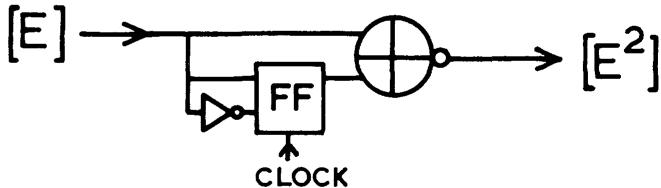
\includegraphics[width=0.6\textwidth, height=7cm, keepaspectratio]{images/879c30ec366d098fb9151a70770fff6be90fbcfc2bb7c014fac61ebfe974c207.jpg}\\
图 4---随机平方器
